\documentclass[10pt,twocolumn]{article}
% Shared two-column preamble for the three research papers.
% Use with: \documentclass[10pt,twocolumn]{article}
% Then in main.tex: % Shared two-column preamble for the three research papers.
% Use with: \documentclass[10pt,twocolumn]{article}
% Then in main.tex: % Shared two-column preamble for the three research papers.
% Use with: \documentclass[10pt,twocolumn]{article}
% Then in main.tex: \input{../../shared/latex/twocolumn_preamble.tex}

\usepackage[margin=0.75in]{geometry}
\usepackage[utf8]{inputenc}
\usepackage[T1]{fontenc}
\usepackage{lmodern}
\usepackage{microtype}
\usepackage{amsmath,amssymb,amsthm}
\usepackage{graphicx}
\usepackage{booktabs}
\usepackage{caption}
\usepackage{subcaption}
\usepackage{hyperref}
\usepackage{url}
\usepackage{xcolor}
\usepackage{algorithm}
\usepackage{algorithmic}
\usepackage{multirow}
\usepackage{titlesec}
\usepackage{authblk}

\hypersetup{colorlinks=true,linkcolor=blue!50!black,citecolor=blue!50!black,urlcolor=blue!50!black}

\titleformat{\section}{\normalfont\large\bfseries}{\thesection}{0.6em}{}
\titleformat{\subsection}{\normalfont\bfseries}{\thesubsection}{0.5em}{}

\captionsetup{font=small,labelfont=bf,skip=4pt}
\setlength{\columnsep}{0.25in}
\setlength{\parskip}{2pt}

\newtheorem{theorem}{Theorem}
\newtheorem{proposition}[theorem]{Proposition}
\newtheorem{definition}[theorem]{Definition}


\usepackage[margin=0.75in]{geometry}
\usepackage[utf8]{inputenc}
\usepackage[T1]{fontenc}
\usepackage{lmodern}
\usepackage{microtype}
\usepackage{amsmath,amssymb,amsthm}
\usepackage{graphicx}
\usepackage{booktabs}
\usepackage{caption}
\usepackage{subcaption}
\usepackage{hyperref}
\usepackage{url}
\usepackage{xcolor}
\usepackage{algorithm}
\usepackage{algorithmic}
\usepackage{multirow}
\usepackage{titlesec}
\usepackage{authblk}

\hypersetup{colorlinks=true,linkcolor=blue!50!black,citecolor=blue!50!black,urlcolor=blue!50!black}

\titleformat{\section}{\normalfont\large\bfseries}{\thesection}{0.6em}{}
\titleformat{\subsection}{\normalfont\bfseries}{\thesubsection}{0.5em}{}

\captionsetup{font=small,labelfont=bf,skip=4pt}
\setlength{\columnsep}{0.25in}
\setlength{\parskip}{2pt}

\newtheorem{theorem}{Theorem}
\newtheorem{proposition}[theorem]{Proposition}
\newtheorem{definition}[theorem]{Definition}


\usepackage[margin=0.75in]{geometry}
\usepackage[utf8]{inputenc}
\usepackage[T1]{fontenc}
\usepackage{lmodern}
\usepackage{microtype}
\usepackage{amsmath,amssymb,amsthm}
\usepackage{graphicx}
\usepackage{booktabs}
\usepackage{caption}
\usepackage{subcaption}
\usepackage{hyperref}
\usepackage{url}
\usepackage{xcolor}
\usepackage{algorithm}
\usepackage{algorithmic}
\usepackage{multirow}
\usepackage{titlesec}
\usepackage{authblk}

\hypersetup{colorlinks=true,linkcolor=blue!50!black,citecolor=blue!50!black,urlcolor=blue!50!black}

\titleformat{\section}{\normalfont\large\bfseries}{\thesection}{0.6em}{}
\titleformat{\subsection}{\normalfont\bfseries}{\thesubsection}{0.5em}{}

\captionsetup{font=small,labelfont=bf,skip=4pt}
\setlength{\columnsep}{0.25in}
\setlength{\parskip}{2pt}

\newtheorem{theorem}{Theorem}
\newtheorem{proposition}[theorem]{Proposition}
\newtheorem{definition}[theorem]{Definition}

\newcommand{\KinV}{1.6}
\newcommand{\KinA}{1.0}
\newcommand{\KinDoor}{4}
\newcommand{\KinPass}{1.2}
\newcommand{\CurveN}{20}
\newcommand{\AnaMiddleLastZero}{11}
\newcommand{\AnaLobbyZero}{7}
\newcommand{\AnaLobbyQuarter}{2}
\newcommand{\AnaLobbyHalf}{2}
\newcommand{\AnaRandomHalf}{6}
\newcommand{\AnaLastHalf}{2}
\newcommand{\AnaMiddleHalf}{10}
\newcommand{\AnaMiddleNine}{2}
\newcommand{\AnaRegretMidHalfLobby}{46}
\newcommand{\AnaRegretMidNineLobby}{163}
\newcommand{\AnaRegretTopNineLobby}{381}
\newcommand{\AnaRegretMidZeroLobby}{3.2}
\newcommand{\AnaBestNineLobby}{14}
\newcommand{\AnaWorstNineLobby}{65}
\newcommand{\AnaBandZeroLobby}{3--10}
\newcommand{\AnaBandZeroRandom}{8--13}
\newcommand{\AnaFortyLobbyHalf}{2}
\newcommand{\AnaFortyRandomZero}{21}
\newcommand{\AnaFortyRegretMidHalf}{67}
\newcommand{\TraValidErr}{2.3}
\newcommand{\TraAlpha}{0.7}
\newcommand{\TraN}{20}
\newcommand{\TraReps}{4}
\newcommand{\TraHorizon}{4}
\newcommand{\TraHZero}{2}
\newcommand{\TraBestZero}{20}
\newcommand{\TraRegMidZero}{83}
\newcommand{\TraRegWorstZero}{210}
\newcommand{\TraHpZero}{9}
\newcommand{\TraHHalf}{2}
\newcommand{\TraBestHalf}{35}
\newcommand{\TraRegMidHalf}{38}
\newcommand{\TraRegWorstHalf}{129}
\newcommand{\TraHpHalf}{4}
\newcommand{\TraHOne}{2}
\newcommand{\TraBestOne}{49}
\newcommand{\TraRegMidOne}{22}
\newcommand{\TraRegWorstOne}{96}
\newcommand{\TraHpOne}{4}
\newcommand{\TraHTwo}{2}
\newcommand{\TraBestTwo}{83}
\newcommand{\TraRegMidTwo}{10}
\newcommand{\TraRegWorstTwo}{82}
\newcommand{\TraHpTwo}{4}
\newcommand{\TraHFour}{11}
\newcommand{\TraBestFour}{160}
\newcommand{\TraRegMidFour}{4}
\newcommand{\TraRegWorstFour}{54}
\newcommand{\TraHpFour}{4}
\newcommand{\TraHiWaitLow}{148}
\newcommand{\TraHiWaitTop}{166}
\newcommand{\TraHiWaitMin}{98}
\newcommand{\TraHiWaitMinFloor}{16}
\newcommand{\TraHiRideLow}{26}
\newcommand{\TraHiRideTop}{80}
\newcommand{\TraHiStopsTop}{5.0}
\newcommand{\TraLastLobbyMass}{30}
\newcommand{\TraLastHFour}{16}
\newcommand{\TraLastLobbyMassHalf}{25}
\newcommand{\StaBestNone}{49}
\newcommand{\StaBestOn}{38}
\newcommand{\StaWalked}{10}
\newcommand{\StaWalkedDownOnly}{7}
\newcommand{\StaWalkedSym}{10}
\newcommand{\StaRegMidNone}{22}
\newcommand{\StaRegMidOn}{51}
\newcommand{\StaH}{2}
\newcommand{\StaAnaZeroNone}{5}
\newcommand{\StaAnaZeroOn}{7}
\newcommand{\StaAnaZeroSym}{7}
\newcommand{\StaAnaZeroDown}{7}
\newcommand{\FleBestOne}{65}
\newcommand{\FleRegMidOne}{16}
\newcommand{\FleHOne}{4}
\newcommand{\FleBandOne}{2--4}
\newcommand{\FleBestTwo}{52}
\newcommand{\FleRegMidTwo}{19}
\newcommand{\FleHTwo}{2}
\newcommand{\FleBandTwo}{2--3}
\newcommand{\FleBestFour}{43}
\newcommand{\FleRegMidFour}{30}
\newcommand{\FleHFour}{3}
\newcommand{\FleBandFour}{2--4}
\newcommand{\RobN}{15}
\newcommand{\RobHZeroZero}{11}
\newcommand{\RobHZeroFour}{13}
\newcommand{\RobHQuarterZero}{5}
\newcommand{\RobHQuarterFour}{11}
\newcommand{\RobHHalfZero}{2}
\newcommand{\RobRegMidZeroZero}{2}
\newcommand{\RobRegMidHalfZero}{27}
\newcommand{\RobRegMidNineOne}{96}
\newcommand{\RobRegTopNineOne}{223}
\newcommand{\RobBandZeroZero}{7--12}
\newcommand{\RobBandQuarterFour}{2--12}
\newcommand{\RobBandWidthQuarterFour}{3}
\newcommand{\RobCellsFloorTwo}{16}
\newcommand{\RobCells}{24}
\newcommand{\RobHalfPlusAllTwo}{yes}
\newcommand{\ArcResidentialH}{2}
\newcommand{\ArcResidentialHp}{2}
\newcommand{\ArcResidentialBest}{28}
\newcommand{\ArcResidentialRegMid}{126}
\newcommand{\ArcResidentialRegTop}{288}
\newcommand{\ArcResidentialBand}{2--2}
\newcommand{\ArcResidentialN}{20}
\newcommand{\ArcResidentialWalked}{5}
\newcommand{\ArcOfficeH}{2}
\newcommand{\ArcOfficeHp}{2}
\newcommand{\ArcOfficeBest}{49}
\newcommand{\ArcOfficeRegMid}{35}
\newcommand{\ArcOfficeRegTop}{102}
\newcommand{\ArcOfficeBand}{2--2}
\newcommand{\ArcOfficeN}{20}
\newcommand{\ArcOfficeWalked}{13}
\newcommand{\ArcHospitalH}{2}
\newcommand{\ArcHospitalHp}{4}
\newcommand{\ArcHospitalBest}{33}
\newcommand{\ArcHospitalRegMid}{8}
\newcommand{\ArcHospitalRegTop}{42}
\newcommand{\ArcHospitalBand}{2--4}
\newcommand{\ArcHospitalN}{12}
\newcommand{\ArcHospitalWalked}{14}


\title{Up or Down? The Optimal Floor to Live On When the Elevator Has to
Come and Get You}
\author[1]{Luis Benvenuto}
\affil[1]{Independent Research}
\date{September 18, 2026}

\begin{document}
\twocolumn[
\maketitle
\begin{@twocolumnfalse}
\begin{abstract}
\noindent Which floor of a building minimises the time you spend getting
around it? The textbook answer is the middle floor: the median minimises
expected distance to a uniformly random destination. But an elevator is not a
distance --- it is a car that has to come and get you from wherever it was
left, most trips start or end at the lobby, other passengers add stops along
the way, and for a floor or two the stairs beat waiting. We formalise the
question as a facility-location problem with a mechanism, solve it in closed
form for one car and no traffic, and validate a discrete-event simulator with
real kinematics, collective control, nearest-car dispatch, Poisson background
traffic, several cars and a stairs option against it (mean error
\TraValidErr\%). The middle-floor intuition survives only when nobody goes to
the lobby and the car waits where you left it (optimum floor
\AnaMiddleLastZero\ of \CurveN); as soon as a quarter of trips go to the lobby
and the car parks there, the optimum drops to floor \AnaLobbyQuarter, and at
a residential mix ($\alpha = 0.9$) the middle floor costs
\AnaRegretMidNineLobby\% more time than the best floor and the top floor
\AnaRegretTopNineLobby\%. Background traffic does not restore the middle: at
moderate load the optimum stays low while the curve flattens (regret of the
middle \TraRegMidTwo\% at 2 passengers/min), and only at saturation does the
optimum drift upward (floor \TraHFour\ at 4/min), because a car sweeping
under load serves the low floors last on its way down. Stairs cut the best
floor's trip time from \StaBestNone\ to \StaBestOn\,s by absorbing
\StaWalked\% of trips, and in a lobby-free building they move the closed-form
optimum up from floor \StaAnaZeroNone\ to \StaAnaZeroOn\ --- but the
up/down asymmetry itself barely matters. A bigger fleet lowers every floor's
time yet makes the choice matter \emph{more} in relative terms (regret of the
middle \FleRegMidOne\% $\to$ \FleRegMidFour\% from one to four cars), because
what remains is ride distance. Across a map of lobby fraction and load,
\RobCellsFloorTwo\ of \RobCells\ settings put the optimum on the lowest
residential floor; the middle floor is within 5\% of optimal only when
lobby trips are rare. The practical rule: if you leave the building more than
you move within it, live as low as you can, and the elevator's parking policy
matters as much as the height.
\end{abstract}
\vspace{1em}
\end{@twocolumnfalse}
]

\section{Introduction}
\label{sec:intro}

Ask which floor of a tall building is the best place to be based --- the flat
you rent, the office you are assigned --- and the reflexive answer is ``the
middle''. The reasoning is the one-median on a line: if destinations are
spread uniformly over the floors, the median floor minimises the expected
distance to them. It is a clean argument, and it is wrong for most buildings,
because it treats the elevator as a distance. An elevator is a mechanism. When
you press the button the car is somewhere else --- at the lobby where the
controller parked it, or wherever it dropped its last passenger --- and it has
to come to you before it can take you anywhere. Most of your trips do not go
to a random floor at all: you leave the building and come back, so the lobby
is the destination or origin of the majority of them. Other people are using
the same car, and each of them adds a stop to your ride. And when you live on
the second floor you do not call the elevator to go down --- you take the
stairs, which is fast, whereas climbing back up is not.

This paper treats the question as a facility-location problem with a
mechanism inside it and answers it quantitatively. We write the expected trip
time of a resident on floor $h$ as a function of the lobby-trip fraction
$\alpha$, the elevator's kinematics (rated speed, acceleration, door and
transfer times), its idle parking policy (return to the lobby, stay put, park
in the middle, or --- the heavy-traffic limit --- be anywhere), the background
passenger rate, the number of cars, and the stairs. For one car and no traffic
the expectation has a closed form; for everything else we run a discrete-event
simulator with collective control and nearest-car dispatch, validated against
the closed form at zero traffic. The objective is the mean trip time, but we
also report the 90th percentile, the \emph{regret} of a floor (how much worse
than the best), and an \emph{indifference band} (the floors within 5\% of the
best), because the practical question is as much ``does it matter?'' as
``which floor?''.

Four findings organise the paper. (i) The middle-floor answer holds only in
the corner where no trip goes to the lobby and the car waits where you left
it; with lobby trips and lobby parking the optimum drops to the lowest
residential floor and the middle floor is far from indifferent. (ii)
Background traffic flattens the curve but does not move the optimum up until
the car is saturated, where an unexpected effect appears: on a loaded car the
low floors are the last to be served on the down sweep, so the optimum drifts
upward. (iii) Stairs shift the optimum upward by absorbing short trips, but
the asymmetry between walking down and climbing up, which we expected to be
the driver, contributes little. (iv) More cars make every floor faster and
make the choice of floor matter \emph{more}, not less, because what is left
of the trip is the ride, which is distance. A map over lobby fraction and load
turns these into a rule of thumb.

\section{Related work}
\label{sec:related}

\paragraph{Elevator traffic analysis.} The engineering of lifts has a mature
literature on round-trip time, handling capacity and interval --- how many
cars a building needs and how long people wait --- codified in CIBSE Guide D
\cite{cibse2020guide} and the treatments of Barney and Al-Sharif
\cite{barney2015elevator} and Strakosch \cite{strakosch2010vertical}. Those
analyses take the population's floor distribution as given and size the
system; we hold the system fixed and ask the passenger's question. The
kinematic model (rated speed, acceleration, door and transfer times) and the
collective-control logic we simulate come from that literature.

\paragraph{Facility location on a line.} Minimising expected distance to a
random point on a line is the 1-median problem, solved by the median of the
destination distribution \cite{hakimi1964optimum}; a fixed ``retrieval''
cost that depends on where a server is parked turns it into a location problem
with a mobile server, close in spirit to the analysis of where to park a
single ambulance or repair vehicle \cite{larson1974hypercube}. Our closed
form is the 1-median with the elevator's parking position added to the
distance.

\paragraph{Stairs versus elevator.} Studies of stair use in buildings measure
walking speeds per flight and the reluctance to climb more than a few floors
\cite{fujiyama2010ascending}; the asymmetry between ascending and descending
speeds is well documented and is what motivated our stairs model.

\paragraph{Simulation of elevator systems.} Discrete-event simulation is the
standard tool for evaluating dispatch and group control
\cite{siikonen1993elevator}; our simulator is a minimal member of that family
(collective control, nearest-car dispatch, capacity), chosen so that it can be
validated exactly against the closed form at zero traffic and so that every
effect we report can be traced to a single mechanism.

\section{Model}
\label{sec:model}

\subsection{Building, car and trips}
Floors are $1..N$ with $1$ the lobby; the resident lives on $h \in \{2..N\}$.
A run of $n$ floors takes $n H / v + v / a$ (per-floor cruise at rated speed
$v = \KinV$\,m/s over $H = 3.3$\,m, plus one start/stop penalty at $a =
\KinA$\,m/s$^2$), which coincides with the exact trapezoidal profile whenever a
single floor suffices to reach rated speed, as it does here; each stop costs a
door cycle of \KinDoor\,s plus \KinPass\,s per passenger transferring. The
resident alternates \emph{outbound} and \emph{return} trips: outbound goes to
the lobby with probability $\alpha$ and otherwise to a uniformly random other
floor $f \ge 2$; the return brings them home. Chaining the trips makes the
origin/destination pairs exactly symmetric --- the car has to fetch you at the
lobby as often as at home --- and gives a precise meaning to ``the car stays
where it last stopped''.

\subsection{Closed form: one car, no traffic}
A trip $(o, d)$ costs the car's approach, one dwell, and the ride,
\begin{equation}
T(o, d \mid c) = \text{run}(|c - o|) + \text{stop} + \text{run}(|o - d|),
\end{equation}
where $c$ is the car's position when called, given by the parking policy:
\emph{lobby} ($c = 1$), \emph{middle} ($c = \lceil (N+1)/2 \rceil$),
\emph{last} ($c = o$: with no other traffic the car is where the resident
got off), or \emph{random} ($c \sim \text{Uniform}\{1..N\}$, the limit in
which traffic has left the car anywhere). $E[T(h)]$ sums over the exact
distribution of chained $(o, d)$ pairs; with stairs available, each pair
costs $\min(\text{elevator}, \text{stairs})$ when the climb is allowed.

\subsection{Discrete-event simulator}
$K$ cars move floor by floor with the same run and stop costs. A car keeps its
direction while there are calls ahead (car calls of passengers on board, hall
calls in its direction), reverses when calls remain only behind, and otherwise
parks (lobby, middle) or stays (last). A new hall call wakes the nearest idle
car; moving cars pick up hall calls they pass in their direction, subject to
capacity (10). Background passengers arrive as a Poisson process at
$\lambda$ per minute with the same lobby fraction, travelling up from or down
to the lobby, or between two floors $\ge 2$. The resident probes the system
every two minutes for \TraHorizon\ hours of building time, with \TraReps\
replications; replication $r$ uses the same background draw for every home
floor (common random numbers), so the curves compare floors rather than
traffic realisations. We record the resident's wait, ride, intermediate stops,
and the cars' positions at the moment of the call.

\subsection{Stairs and objective}
Stairs cost $t_{\downarrow}$ per floor descended and $t_{\uparrow}$ per floor
climbed (defaults 10 and 15\,s), with a maximum climb the resident is willing
to make (3 floors); the resident walks when the stairs time is below the
\emph{expected} elevator time for the trip (they do not know where the car
is). For a home floor we report the mean trip time, its 90th percentile, the
regret $E[T(h)] - \min_{h'} E[T(h')]$ in percent, and the indifference band of
floors within 5\% of the best.

\section{One car, no traffic: the closed form}
\label{sec:closed}

\begin{figure*}[t]
\centering
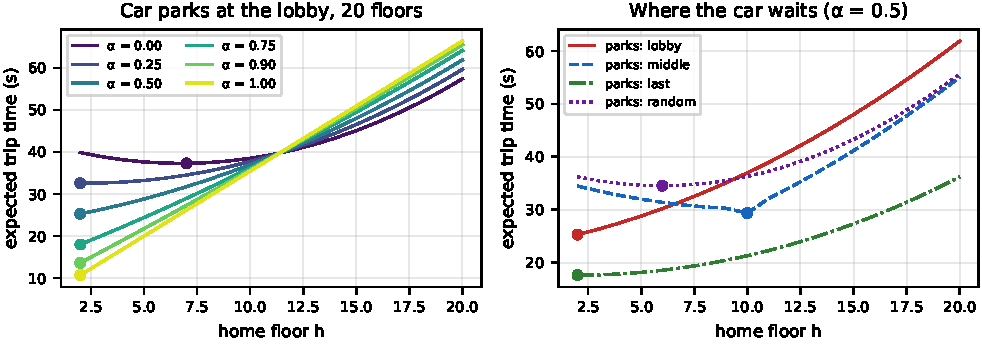
\includegraphics[width=\textwidth]{figures/curves.pdf}
\caption{Closed-form expected trip time versus home floor in a \CurveN-floor
building. Left: the car parks at the lobby; each curve is a lobby-trip
fraction $\alpha$, dots mark the optimum. Right: $\alpha = 0.5$ under the four
parking policies. The middle-floor intuition needs both no lobby trips and a
car that waits where you left it.}
\label{fig:curves}
\end{figure*}

Figure~\ref{fig:curves} is the whole argument in two panels. With no lobby
trips ($\alpha = 0$) and a car that stays where it last stopped, the wait is a
door cycle and only the ride counts: the optimum is the median floor
(\AnaMiddleLastZero\ of \CurveN) and the curve is flat around it. Change
either assumption and the optimum moves. If the car parks at the lobby, even
with $\alpha = 0$ the approach time grows with $h$ and the optimum slides to
floor \AnaLobbyZero, with an indifference band of floors
\AnaBandZeroLobby. If a quarter of trips go to the lobby, the optimum is
floor \AnaLobbyQuarter\ --- the lowest residential floor --- and it stays
there for every larger $\alpha$: at $\alpha = 0.5$ the middle floor costs
\AnaRegretMidHalfLobby\% more than the best, at $\alpha = 0.9$ it costs
\AnaRegretMidNineLobby\% more (\AnaBestNineLobby\,s versus a top floor at
\AnaWorstNineLobby\,s, \AnaRegretTopNineLobby\% worse).

The right panel isolates the mechanism. Parking at the middle floor makes the
middle floor optimal at $\alpha = 0.5$ (floor \AnaMiddleHalf), because the
approach is now shortest there; the random-position limit gives floor
\AnaRandomHalf\ with a wide band (\AnaBandZeroRandom\ at $\alpha = 0$),
because the approach no longer depends on $h$ and only the lobby trips pull
the optimum down; and the stay-put policy gives floor \AnaLastHalf\ because
the resident's own lobby trips leave the car at the lobby half the time. The
parking policy, which the resident never chooses, moves the answer as much
as the lobby fraction does. The picture scales with height: in a 40-floor
building at $\alpha = 0.5$ the optimum with lobby parking is still floor
\AnaFortyLobbyHalf\ and the middle floor's regret is
\AnaFortyRegretMidHalf\%, while the random-position, no-lobby case puts it at
floor \AnaFortyRandomZero, the median.

\section{Traffic, stairs and fleet}
\label{sec:traffic}

\begin{figure*}[t]
\centering
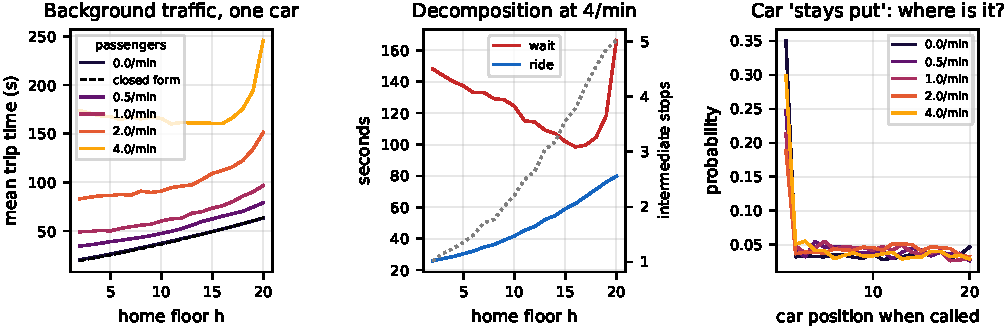
\includegraphics[width=\textwidth]{figures/traffic.pdf}
\caption{One car, lobby parking, $\alpha = \TraAlpha$, \TraN\ floors. Left:
mean trip time versus home floor for background rates from 0 to 4 passengers
per minute; the closed form (dashed) matches the simulator at zero traffic.
Middle: decomposition at 4/min --- the wait falls with height while the ride
and the number of intermediate stops rise. Right: where the car is when the
resident calls under the stay-put policy: the lobby dominates at every load.}
\label{fig:traffic}
\end{figure*}

\paragraph{Validation.} At zero traffic the simulator reproduces the closed
form to \TraValidErr\% mean relative error over all floors
(Figure~\ref{fig:traffic}, left), with the residual coming from the car
occasionally being caught mid-return to its parking floor.

\paragraph{Traffic flattens, then inverts.} Adding background passengers
raises every floor's time and compresses the curve: the regret of the middle
floor falls from \TraRegMidZero\% at zero traffic to \TraRegMidOne\% at
1/min and \TraRegMidTwo\% at 2/min, while the optimum stays at floor
\TraHTwo. At 4 passengers per minute a single car serving 20 floors is
saturated (best mean \TraBestFour\,s, of which most is waiting), and the
optimum jumps to floor \TraHFour\ with a middle-floor regret of only
\TraRegMidFour\%. The middle panel shows why. Under load the car sweeps the
building like a bus; a resident on a low floor who wants to go down is the
\emph{last} stop of the down sweep, so their wait (\TraHiWaitLow\,s on floor
2) exceeds that of a resident on floor \TraHiWaitMinFloor\
(\TraHiWaitMin\,s), and only the very top floor, served at the reversal, waits
longer still (\TraHiWaitTop\,s). Against that, the ride grows with height
(\TraHiRideLow\,s to \TraHiRideTop\,s) and collects up to \TraHiStopsTop\
intermediate stops. The two slopes nearly cancel over the middle of the
building, which is what ``it does not matter'' looks like in a saturated
system --- and the p90-optimal floor (\TraHpFour) remains low, because the
tail is made of the sweeps you miss.

\paragraph{Where the car actually is.} The right panel measures the stay-put
policy under traffic: the car is at the lobby \TraLastLobbyMassHalf\% of the
time at 0.5/min and \TraLastLobbyMass\% at 4/min, with the rest spread
almost uniformly. The stay-put policy is, in practice, a mixture of lobby
parking and the random-position limit --- which is why its optimum behaves
like the lobby-parking one at low load and drifts up (floor \TraLastHFour\ at
4/min) at high load.

\begin{figure}[t]
\centering
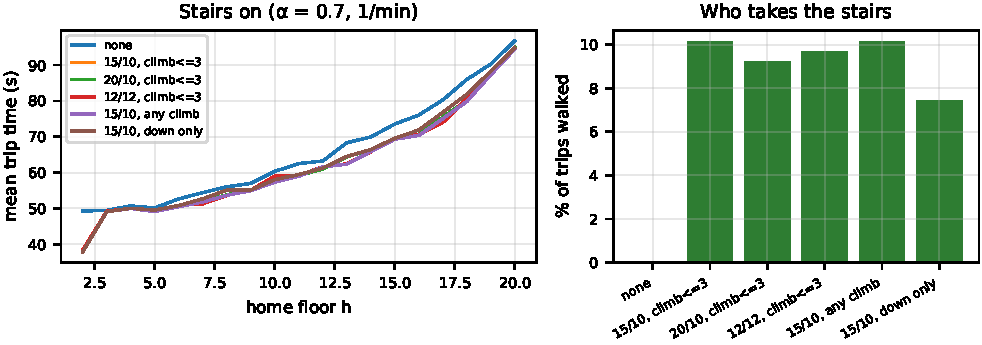
\includegraphics[width=\columnwidth]{figures/stairs.pdf}
\caption{Stairs at $\alpha = 0.7$, 1 passenger/min, one car. Left: mean trip
time by home floor for each stairs variant; right: fraction of trips walked.}
\label{fig:stairs}
\end{figure}

\paragraph{Stairs.} With the stairs available (15\,s up, 10\,s down, at most
three floors climbed) the best floor's mean time drops from \StaBestNone\ to
\StaBestOn\,s and \StaWalked\% of trips are walked, almost all of them the
one- and two-floor hops of a low-floor resident (Figure~\ref{fig:stairs}).
The optimum stays at floor \StaH\ at this lobby fraction, and the middle
floor's regret \emph{rises} from \StaRegMidNone\% to \StaRegMidOn\%, because
the stairs help the low floors most. The asymmetry we expected to matter does
not: a symmetric 12/12\,s stairs walks \StaWalkedSym\% of trips and a
descend-only resident \StaWalkedDownOnly\%, with the same optimum. Stairs do
move the optimum upward in the closed form when lobby trips are absent ---
from floor \StaAnaZeroNone\ to \StaAnaZeroOn\ of 15 with lobby parking ---
but they do so equally with symmetric costs (\StaAnaZeroSym) and with
descending only (\StaAnaZeroDown): the shift comes from the stairs absorbing
the short trips that the lobby-parked car served badly, not from the cost of
climbing.

\begin{figure}[t]
\centering
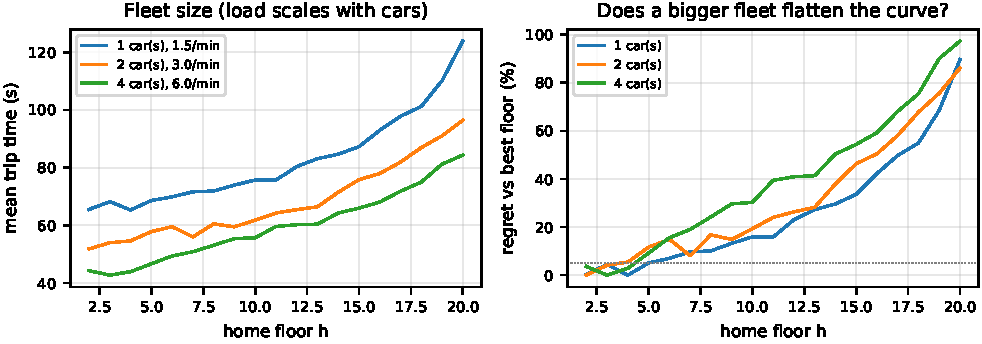
\includegraphics[width=\columnwidth]{figures/fleet.pdf}
\caption{One, two and four cars with a background load that scales with the
fleet (1.5 passengers/min per car). Left: mean trip time; right: regret
relative to the best floor. A bigger fleet lowers every floor and steepens the
curve in relative terms.}
\label{fig:fleet}
\end{figure}

\paragraph{Fleet.} Adding cars at constant load per car lowers the best
floor's time from \FleBestOne\,s (one car) to \FleBestTwo\,s (two) and
\FleBestFour\,s (four) --- and raises the middle floor's regret from
\FleRegMidOne\% to \FleRegMidTwo\% and \FleRegMidFour\%
(Figure~\ref{fig:fleet}). More cars remove waiting, and waiting was the part
of the trip that did not depend much on $h$; what remains is the ride, which
is distance. The intuition that a well-served building makes the floor
irrelevant is backwards: it makes the floor a larger share of what you feel.

\section{The map, and does it matter?}
\label{sec:map}

\begin{figure*}[t]
\centering
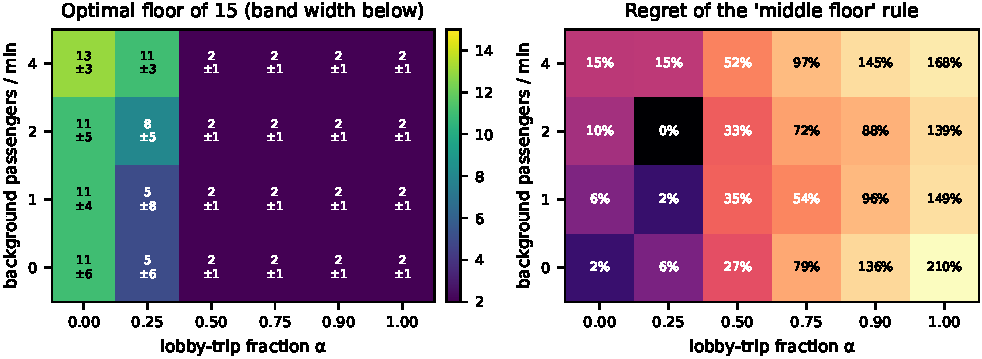
\includegraphics[width=\textwidth]{figures/map.pdf}
\caption{\RobN-floor building, one car parked at the lobby, stairs on. Left:
optimal floor over lobby-trip fraction and background rate, with the width of
the 5\% indifference band beneath each value. Right: regret of the
middle-floor rule in the same cells.}
\label{fig:map}
\end{figure*}

Figure~\ref{fig:map} puts the pieces on one grid. In \RobCellsFloorTwo\ of
\RobCells\ cells --- every cell with $\alpha \ge 0.5$ --- the optimum is the
lowest residential floor, and its indifference band is a single floor. The
middle floor is competitive only along the left edge: at $\alpha = 0$ the
optimum is the median (\RobHZeroZero\ at zero traffic, band
\RobBandZeroZero) drifting up to \RobHZeroFour\ under saturation; at $\alpha =
0.25$ it is floor \RobHQuarterZero\ at zero traffic and rises with load to
\RobHQuarterFour, with a band that spans \RobBandQuarterFour\ at 4/min --- the
one regime where the honest answer is ``it does not matter''. Everywhere to
the right the middle-floor rule costs tens to hundreds of percent
(\RobRegMidHalfZero\% at $\alpha = 0.5$, \RobRegMidNineOne\% at $\alpha =
0.9$ with 1/min, where the top floor costs \RobRegTopNineOne\%).

\begin{figure*}[t]
\centering
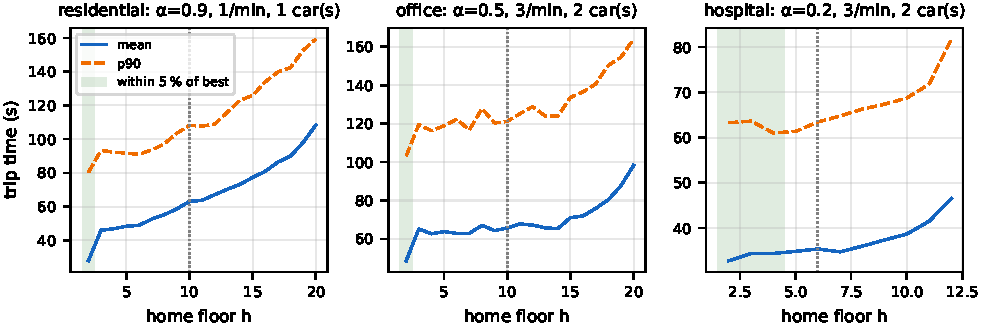
\includegraphics[width=\textwidth]{figures/regret.pdf}
\caption{Three archetypes with stairs on: mean and 90th-percentile trip time
by home floor, the 5\% indifference band (shaded) and the middle floor
(dotted).}
\label{fig:arch}
\end{figure*}

Three archetypes make it concrete (Figure~\ref{fig:arch}). A
\emph{residential} tower (\ArcResidentialN\ floors, $\alpha = 0.9$, one car,
1/min): optimum floor \ArcResidentialH, band \ArcResidentialBand, the middle
floor \ArcResidentialRegMid\% worse and the top floor
\ArcResidentialRegTop\% worse; the p90-optimal floor is the same. An
\emph{office} (\ArcOfficeN\ floors, $\alpha = 0.5$, two cars, 3/min): optimum
\ArcOfficeH, middle-floor regret \ArcOfficeRegMid\%, \ArcOfficeWalked\% of
trips walked. A \emph{hospital}-like building (\ArcHospitalN\ floors, $\alpha
= 0.2$, two cars, 3/min, cars parked mid-building): optimum \ArcHospitalH\
with a band of \ArcHospitalBand, middle-floor regret \ArcHospitalRegMid\%,
p90-optimal floor \ArcHospitalHp\ --- the one case where the floors are close
to interchangeable and the tail, not the mean, should pick.

The rule of thumb that survives all of this: count how often you leave the
building against how often you move within it. If leaving dominates, the
lowest floor you can get wins by a wide margin, the elevator's parking policy
is the next most important thing, and the stairs make the low floor better
still. If moving within dominates and the cars are busy, live anywhere from
the middle up and stop worrying.

\section{Limitations and conclusion}
\label{sec:conclusion}

\paragraph{Limitations.} The building is a stylised one: uniform floor
population, a single lobby, no express zones or sky lobbies, no time-of-day
peaks, and a resident whose destinations are uniform over the other floors.
The simulator implements collective control with nearest-car dispatch, not a
modern destination-dispatch group controller, and its parking policies are
the three textbook ones; real controllers learn where to park, which would
move our ``lobby'' and ``random'' limits toward each other. The kinematics are
mid-rise values (\KinV\,m/s), so the floor-by-floor run model coincides with
the trapezoid; high-speed cars would need the exact profile, which the code
provides. The stairs rule is deterministic on expectations and ignores effort,
carrying things, and the building's actual stair placement. The resident's
probing trips are frequent enough to perturb a loaded single car slightly.
All of these are configuration knobs, and the accompanying full-scale
configuration widens every grid.

\paragraph{Conclusion.} The middle floor is the right answer to a question
nobody asks --- where to be if every trip is to a random floor and the
elevator is waiting outside your door. Once the elevator has to come and get
you, the answer depends on where it waits; once most trips go to the lobby,
the answer is the lowest floor you can get, by a margin that grows with the
building and with the number of cars. Traffic blurs the curve but does not
move the optimum up until the car is saturated, and there the effect that
lifts it is a queueing one (the low floors are served last on the down sweep)
rather than a geometric one. Stairs make the low floors better still and shift
a lobby-free building's optimum upward by absorbing short trips, but the
cost of climbing is not what does it. And the sense in which ``it does not
matter'' is precise: the indifference band is one floor wide wherever lobby
trips are common, and spans most of the building only where they are rare
and the car is busy. Up or down? Down, unless you never leave.


\FloatBarrier
\bibliographystyle{plain}
\bibliography{references}

\end{document}
